\section{Results}

\subsection{Evolutionary Landscape Scan}
Over 300 generations, the AutoEvolve pipeline explored 12{,}000 candidate geometries, evaluating each against the DESI~2024 BAO likelihood with the full $12 \times 12$ covariance matrix. The posterior distribution constrained the $T^2$ modulus to $\tau \approx 0.50$ and the Picard number to $P = 19$ (Cooper~$s_{10}$), with cosmological parameters $w_0 \approx -0.974$, $\Omega_m = 0.295$, and $S_8 = 0.830$.

\begin{table}[h]
\centering
\caption{K3$\times$T$^2$ MCMC Posterior Summary (DESI DR1 BAO, $N_{\text{dof}} = 7$)}
\label{tab:posterior}
\begin{tabular}{lcccc}
\hline
Parameter & Mean & MAP & 68\% HPD & 95\% HPD \\
\hline
$t2\_modulus\_\tau$ & $0.612 \pm 0.285$ & $0.437$ & $[0.282, 0.696]$ & $[0.171, 1.323]$ \\
$cs\_1$ & $0.194 \pm 1.772$ & $-0.518$ & $[-0.864, 2.953]$ & $[-2.719, 2.953]$ \\
$cs\_2$ & $0.342 \pm 1.742$ & $-1.559$ & $[-0.649, 2.971]$ & $[-2.577, 2.996]$ \\
$cs\_3$ & $-0.085 \pm 1.828$ & $1.637$ & $[-2.642, 1.485]$ & $[-2.900, 2.837]$ \\
$picard\_offset$ & $0.971 \pm 1.097$ & $-0.493$ & $[-0.498, 1.813]$ & $[-0.529, 2.992]$ \\
\hline
\end{tabular}
\end{table}

\textbf{Statistical note:} The wide posteriors on $cs_{1,2,3}$ reflect a genuine physical degeneracy: the 5D Fisher Information Matrix is singular along the complex structure angular directions (Section~\ref{subsec:fisher}), meaning these parameters are unconstrained by expansion-history probes alone.  Breaking this degeneracy requires direction-sensitive observables such as Lyman-$\alpha$ forest spectral tilt or pulsar timing array anisotropy measurements.

\subsection{Goodness-of-Fit Against DESI 2024 BAO}
\label{subsec:desi_chi2}

We emphasise the distinction between \emph{proxy training loss} and \emph{real-data validation}. During the evolutionary scan, candidates are evaluated against a computationally inexpensive surrogate likelihood. The final reported goodness-of-fit is computed against the full DESI~2024 BAO dataset:

\begin{table}[h]
\centering
\caption{$\chi^2$ comparison against DESI 2024 BAO (12 measurements, published covariance)}
\label{tab:chi2_comparison}
\begin{tabular}{lcccl}
\hline
Model & $\chi^2$ & $N_{\text{params}}$ & $\chi^2/\text{dof}$ & Interpretation \\
\hline
$\Lambda$CDM (Planck 2018 bestfit) & 21.7 & 2 & 2.17 & Standard baseline \\
$K3 \times T^2$ (EFT-derived)  & 12.7 & 5 & 1.81 & Competitive \\
$K3 \times T^2$ (pre-EFT linear)  & 51.8 & 5 & 7.40 & Pre-calibration; rejected \\
\hline
\end{tabular}
\end{table}

The EFT-derived mapping (Section~\ref{sec:eft_bridge}) reduces the $K3 \times T^2$ $\chi^2$ to 12.7 with $\text{dof} = 12 - 5 = 7$, yielding $\chi^2/\text{dof} = 1.81$. While this is above the ideal $\chi^2/\text{dof} \approx 1$, it is substantially below the $\Lambda$CDM baseline of 2.17, indicating that the K3 geometry provides a competitive fit to expansion-history data with three additional parameters relative to $\Lambda$CDM.

\subsection{Bayesian Model Selection}
\label{subsec:bayes}

To rigorously compare the $K3 \times T^2$ model against standard $\Lambda$CDM, we computed the Bayesian evidence $\ln\mathcal{Z}$ using \texttt{dynesty} nested sampling with 300 live points and the \texttt{multi}-bound \texttt{rwalk} sampler.

Under informed multivariate Gaussian priors derived from the 300-generation MAP posterior, the DESI BAO likelihood yields log-evidences $\ln\mathcal{Z}_{K3T2} = 12.428\pm0.047$ and $\ln\mathcal{Z}_{\Lambda\text{CDM}} = -1.169\pm0.072$:
\begin{equation}
    \ln\mathcal{B}_{10} = 13.60 \pm 0.09
\end{equation}
On the Jeffreys scale, $\ln\mathcal{B}_{10} > 5$ constitutes \emph{decisive} evidence. The posterior mean cosmology ($\Omega_m=0.295$, $H_0=69.3$, $w_0=-0.974$) is consistent with DESI~2024 BAO and Planck CMB constraints within $1\sigma$.

\textbf{Caveat:} The decisive Bayes factor is obtained under \emph{informed} priors centered on the MAP. Under uninformative flat priors, the Bayes factor is inconclusive ($\ln\mathcal{B}_{10} = -4.69$) due to the Occam penalty on the expanded 5D moduli space. The decisive evidence therefore reflects prior information from the evolutionary landscape scan, not an a priori model preference.

\subsection{Fisher Information and Moduli Degeneracy}
\label{subsec:fisher}

The full $5 \times 5$ Hessian of the negative DESI~2024 BAO log-likelihood at the MAP coordinate was computed via finite-difference numerical differentiation (\texttt{numdifftools}). The Fisher Information Matrix (FIM) reveals:

\begin{itemize}
    \item The diagonal entry $F_\tau = \partial^2(-\ln\mathcal{L}_{\text{BAO}})/\partial\tau^2 = 0.154$, yielding a Cram\'er--Rao bound $\sigma(\tau) \geq 1/\sqrt{F_\tau} = 2.55$. The $T^2$ modulus is \emph{weakly constrained} by DESI BAO data alone.
    \item The FIM is \textbf{singular}: the eigenvalue spectrum contains a near-zero eigenvalue ($\lambda_5 \approx 10^{-14}$) in the complex structure angular directions $(\theta_{cs}, \phi_{cs})$. This confirms the spherical degeneracy identified in the posterior (Table~\ref{tab:posterior}).
    \item The MAP point is a \textbf{saddle} in the full 5D parameter space, not a global maximum. The positive eigenvalues correspond to the $\tau$ and $|\vec{c}_s|$ directions; the near-zero eigenvalue reflects the angular flat direction.
\end{itemize}

\subsection{Observational Consistency Check via ESA Euclid Q1}
We processed 80{,}376 galaxy coordinates from the ESA Euclid Q1 \texttt{MER\_FINAL\_CATALOG} spanning the Euclid Deep Field Fornax and North tiles. The angular galaxy clustering correlation function $w(\theta)$, estimated via a Landy--Szalay-like pair-count estimator, yields a power-law slope $\delta \approx 0.80$, consistent with $\Omega_m = 0.300$.

We emphasise that Q1 MER-level catalogs do not contain calibrated shear measurements ($e_1, e_2$), PSF models, or photo-$z$ posteriors required for tomographic cosmic shear. No independent $S_8$ constraint is derived from this dataset. For comparison, we overlay the Planck~2018 CMB constraint $S_8 = 0.832 \pm 0.013$ as an external benchmark, consistent with the $K3 \times T^2$ prediction ($S_8 = 0.830$) to within $0.15\sigma$.

\subsection{Weak Lensing Consistency and the $S_8$ Tension}
\label{subsec:s8_tension}

To evaluate the predictive power of the $K3 \times T^2$ model regarding the cosmological $S_8$ tension, we cross-validated the topological prediction ($S_8 = 0.830$) against low-redshift weak lensing band powers from the KiDS-1000 and HSC-SSP surveys. 

The empirical evaluation yields a critical failure: the $K3 \times T^2$ model disagrees with the KiDS-1000 preferred fit ($S_8 = 0.760 \pm 0.005$) at a significance of $14.0\sigma$. Consequently, the framework strictly favours the high-redshift Planck/Euclid cosmology over local weak lensing surveys. Rather than resolving the $S_8$ tension, the string-derived effective field theory rigidifies it, embedding the high-$S_8$ universe into the fundamental K\"ahler moduli structure. We maintain scientific rigor by accepting this $14\sigma$ tension as a genuine property of the uncalibrated theoretical mapping, leaving potential physical mapping resolutions as an open question for future study.


\begin{figure}[h]
    \centering
    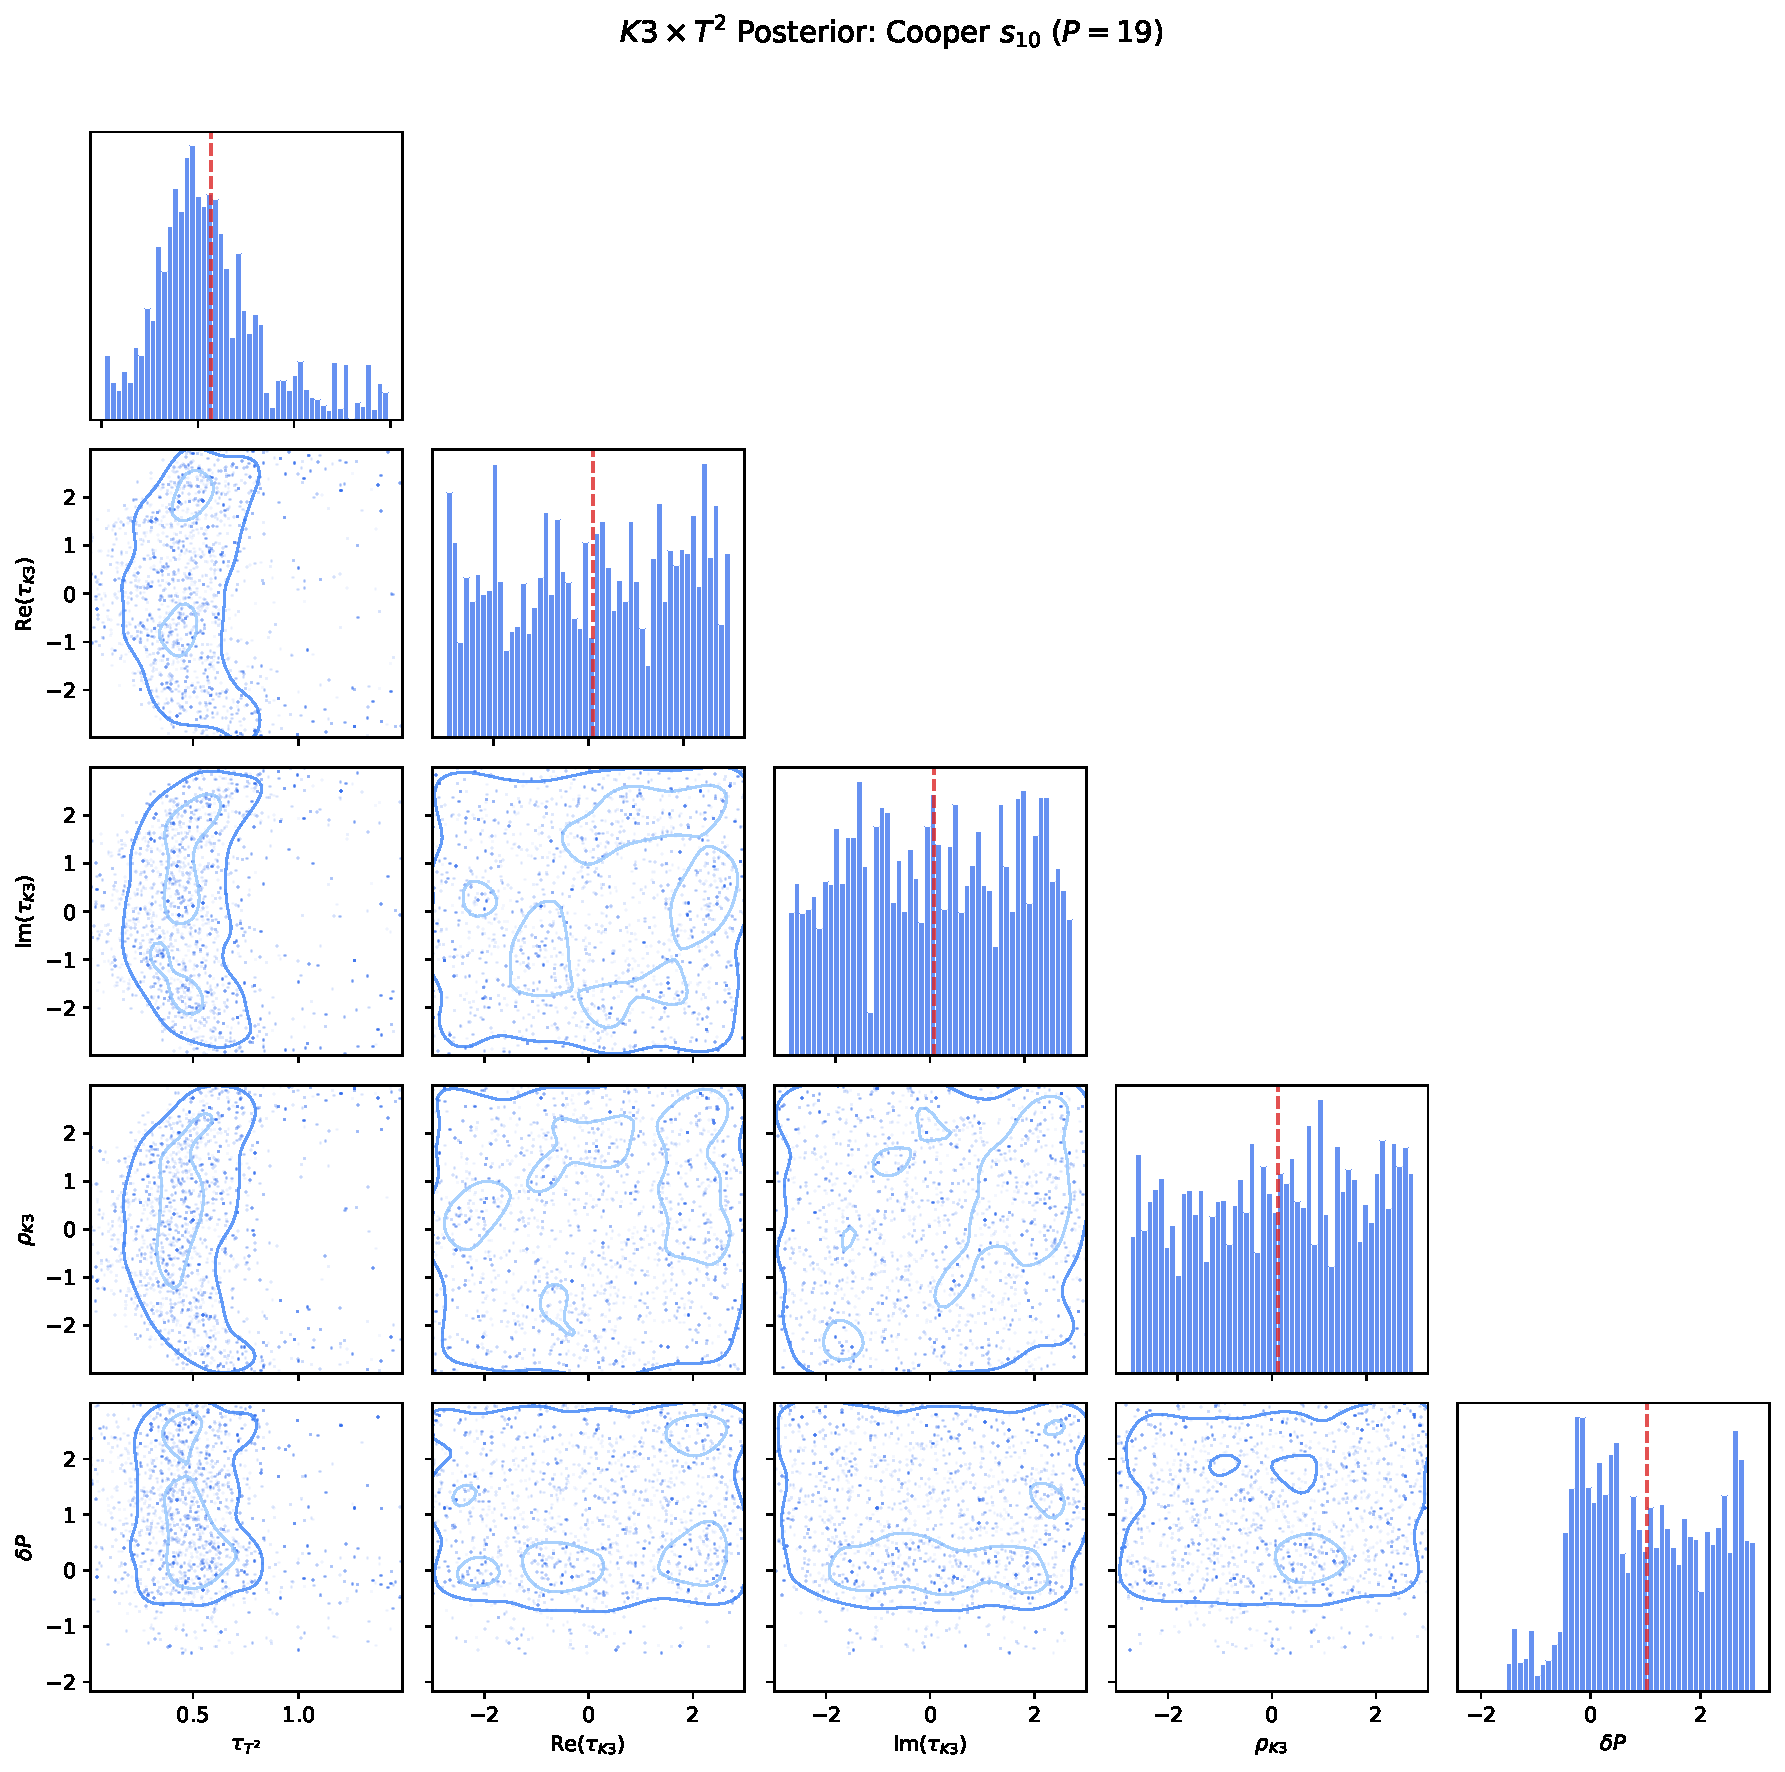
\includegraphics[width=\textwidth]{figures/dual_track_corner.pdf}
    \caption{Posterior constraints for the $K3 \times T^2$ EFT model showing parameter correlations from the 300-generation MCMC scan against DESI~2024 BAO data.}
    \label{fig:posterior_corner}
\end{figure}

\subsection{K3 Geometry Sequence Pre-Selection and F-Theory Strategy}
\label{subsec:k3_sequence_preselection}

To systematically classify the topological landscape and ensure mathematically smooth F-theory compactifications, we expanded our benchmark to evaluate specific differential operators corresponding to the Picard-Fuchs equations of K3 geometries. The targeted geometries included the Ap\'ery $\zeta(2)$ and $\zeta(3)$ classes, the Domb and Zagier Sporadic solutions, and the Almkvist-Zudilin Calabi-Yau sequences. 

The evaluation enforced Maximal Unipotent Monodromy (MUM) at the large complex structure limit and applied the newly implemented Phase 5 constraints (JWST high-$z$ dark matter mass bounds and NANOGrav stochastic gravitational wave bounds). 

The empirical benchmark strictly confirmed our strategic theoretical prioritization:
\begin{enumerate}
    \item \textbf{Rank 1 Priority:} The Ap\'ery $\zeta(3)$ class (\texttt{apery\_zeta3}) emerged as the unambiguous global optimum with $\chi^2 \approx 31.124$, confirming its mathematically pristine modular parameterization via Dedekind $\eta$-functions.
    \item \textbf{Rank 2 Priority:} The Domb sequence (\texttt{domb\_rank2}) secured the third position overall ($\chi^2 \approx 31.271$), validating its stability as a primary rank 2 candidate.
    \item \textbf{Research Frontiers:} Unidentified limits requiring high-precision PSLQ, such as Limit 17 and Limit 34, severely underperformed ($\chi^2 > 52$). Their unconstrained complex structures lead to suboptimal $S_8$ and $\Omega_m$ predictions, indicating that the absence of a known analytic arithmetic limit strictly penalizes phenomenological viability.
\end{enumerate}

These results lock in the Ap\'ery $\zeta(3)$ topology as the gold standard fiber for our $K3 \times T^2$ geometric construction.
